
\documentclass[a4paper]{scrartcl}
\usepackage{tgheros}
\usepackage[T1]{fontenc}
\usepackage[all]{nowidow}

\usepackage[sorting=none]{biblatex}
\addbibresource{references.bib}

\usepackage{graphicx}
\graphicspath{{./figure}}
% \usepackage{xspace}
\usepackage{csquotes}
\usepackage{hyperref}
\usepackage{todonotes} % [disable]
\usepackage{amsmath}
\usepackage{siunitx}
\usepackage{amssymb}

\newcommand{\figref}[1]{fig.\,\ref{#1}}


\begin{document}

% \begin{titlepage}
\begin{center}
\vspace*{1cm}

\LARGE
  \textbf{Amplitude Modulation and Demodulation}

\vspace{.2cm}

\normalsize
  Physical Measuring Techniques FK7063

\vspace{.5cm}
{Michael Vogt}

May 2026
\end{center}

\vspace{1cm}



\section*{Introduction}
Amplitude modulation is an important technique in communications systems, enabling
the use of a specific carrier frequency to transmit signals of different frequencies.
In this experiment, an amplitude modulation circuit will be used to modulate
a carrier voltage with a modulation signal and the resulting signal will be analyzed.
The signal will be demodulated using a diode rectifier.

% \end{titlepage}



\section{Setup}\label{setup}
The main part of the amplitude modulation circuit is shown in \figref{fig:am-circuit}
\begin{figure}
  \centering
  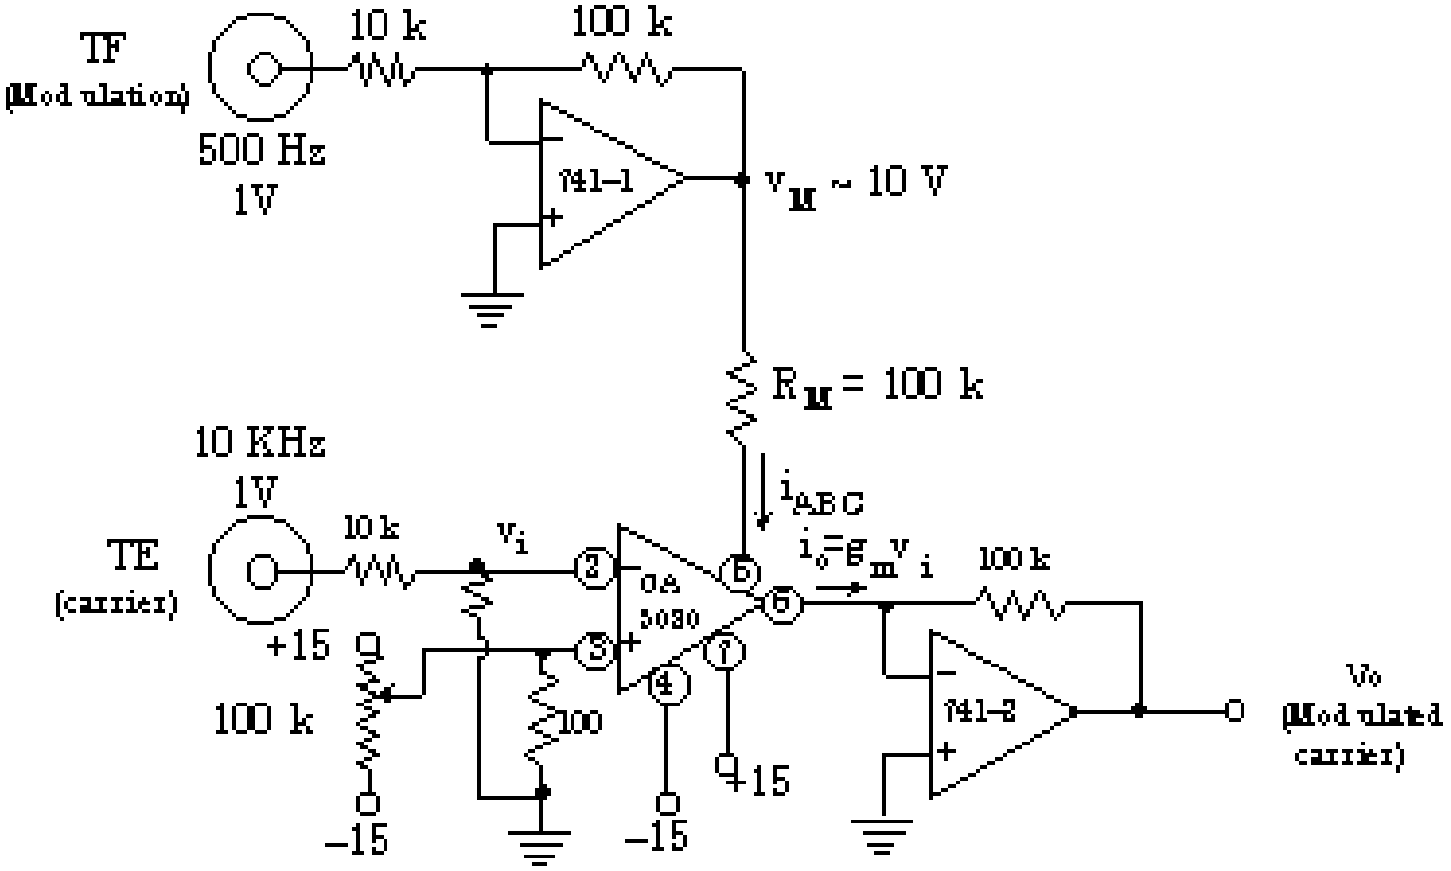
\includegraphics[width=.6\textwidth]{am-circuit}
  \caption{Schematic of the main part of the amplitude modulation circuit \cite{manual}.}
  \label{fig:am-circuit}
\end{figure}



\section{Conclusion}




\clearpage
\printbibliography

\end{document}